% --------------------------------------------------------------------------------------------------
% Section: Overview of Lung Cancer
% --------------------------------------------------------------------------------------------------
\section{Overview of Lung Cancer}

% --------------------------------------------------------------------------------------------------
% Subsection: Definition and Classification
% Introduces lung cancer and its two main categories
% --------------------------------------------------------------------------------------------------
\subsection{Definition and Classification}
Lung cancer is a malignant tumor characterized by the uncontrolled growth of abnormal cells in one 
or both lungs. These abnormal cells do not carry out the functions of normal lung cells and do not 
develop into healthy lung tissue. Instead, they divide rapidly and form tumors that can interfere 
with the lung’s primary function of providing oxygen to the body via the bloodstream. Without 
treatment, these tumors can spread within the lungs and to other parts of the body, further 
impairing lung function and overall health.

% Two primary classifications based on cell type
Lung cancer is broadly classified into two main categories based on the appearance of the cancer 
cells under a microscope:
\begin{itemize}
    % Non-small cell lung cancer is more common
    \item \textbf{Non-Small Cell Lung Cancer (NSCLC)}: This is the most common type, accounting for 
    approximately 85\% of all lung cancer cases.

    % Small cell lung cancer is less common but more aggressive
    \item \textbf{Small Cell Lung Cancer (SCLC)}: Less common and more aggressive, accounting for 
    about 15\% of cases.
\end{itemize}
% Importance of classification for treatment and prognosis
These classifications are crucial as they guide the therapeutic strategy and have different 
prognosis and biological behaviors.

% --------------------------------------------------------------------------------------------------
% Subsection: Histological Types of NSCLC and SCLC
% --------------------------------------------------------------------------------------------------
\subsection{Histological Types: NSCLC vs. SCLC}

% Introduction to NSCLC subtypes
\textbf{NSCLC} comprises several histological subtypes, each with distinct pathological and clinical 
characteristics:

\begin{itemize}
    % Adenocarcinoma: most common NSCLC subtype
    \item \textbf{Adenocarcinoma}: The most prevalent subtype of NSCLC, particularly among 
    non-smokers and younger individuals. It originates from glandular epithelial cells and is 
    frequently located in the lung periphery. Adenocarcinomas exhibit significant histological 
    heterogeneity and may present mixed patterns, such as acinar, papillary, solid, or 
    bronchioloalveolar features. The WHO/IASLC classification recognizes several variants, including 
    mucinous, fetal, and signet ring types. \cite{nlm2025}
\end{itemize}

% CT scan image of adenocarcinoma
\vspace{1em}
\begin{center}
    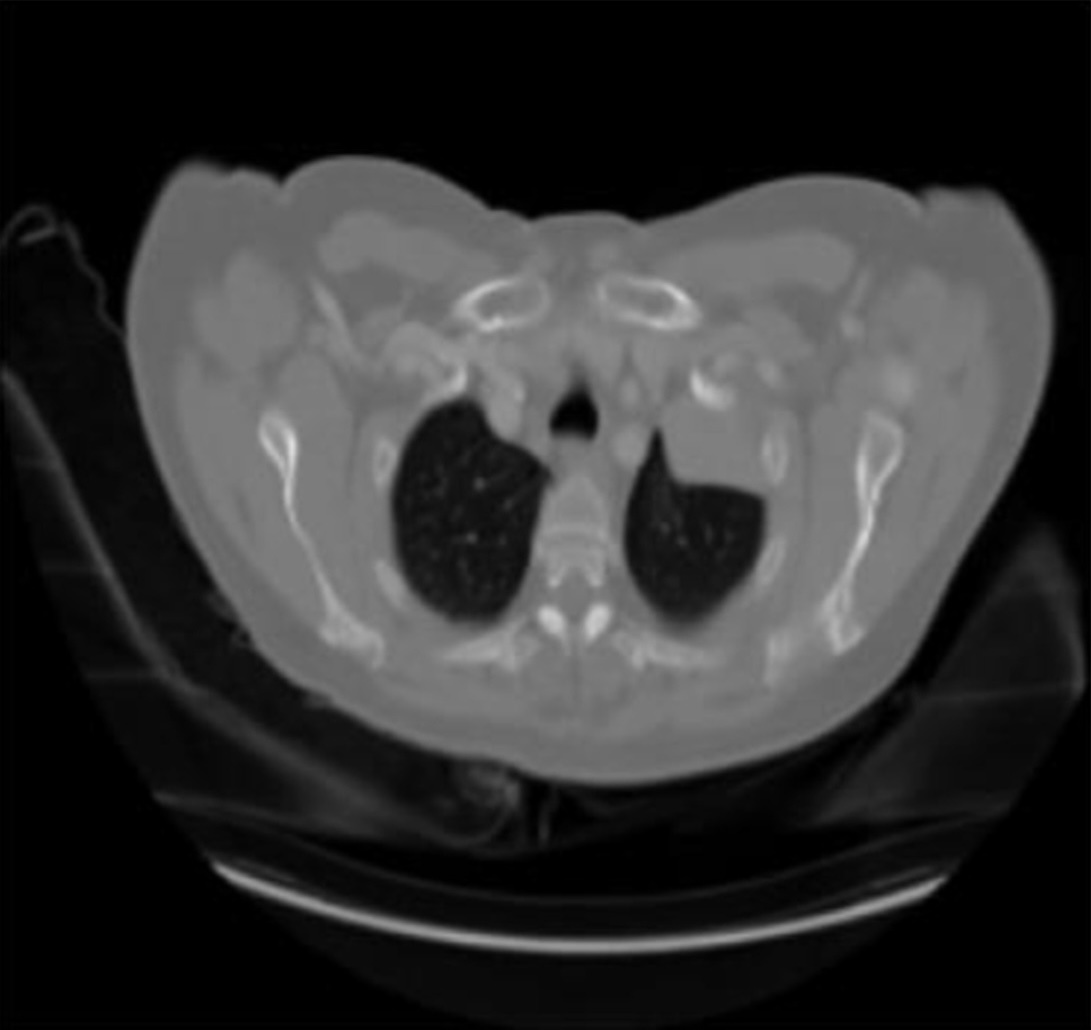
\includegraphics[width=0.5\textwidth]{../assets/01-overview/lc-adc-ct.jpeg}

    \small\textit{CT scan of patient diagnosed with lung Adenocarcinoma. \cite{SHATNAWI2025100188}}
\end{center}
\vspace{1em}

\begin{itemize}
    % Squamous Cell Carcinoma: related to smoking
    \item \textbf{Squamous Cell Carcinoma}: Commonly found in the central airways, this subtype 
    arises from squamous epithelial cells and is strongly associated with tobacco smoking. It is 
    characterized histologically by keratinization and intercellular bridges. The incidence of 
    squamous cell carcinoma has declined in recent years due to reduced smoking rates. 
    \cite{nlm2025}
\end{itemize}

% CT scan image of squamous cell carcinoma
\vspace{1em}
\begin{center}
    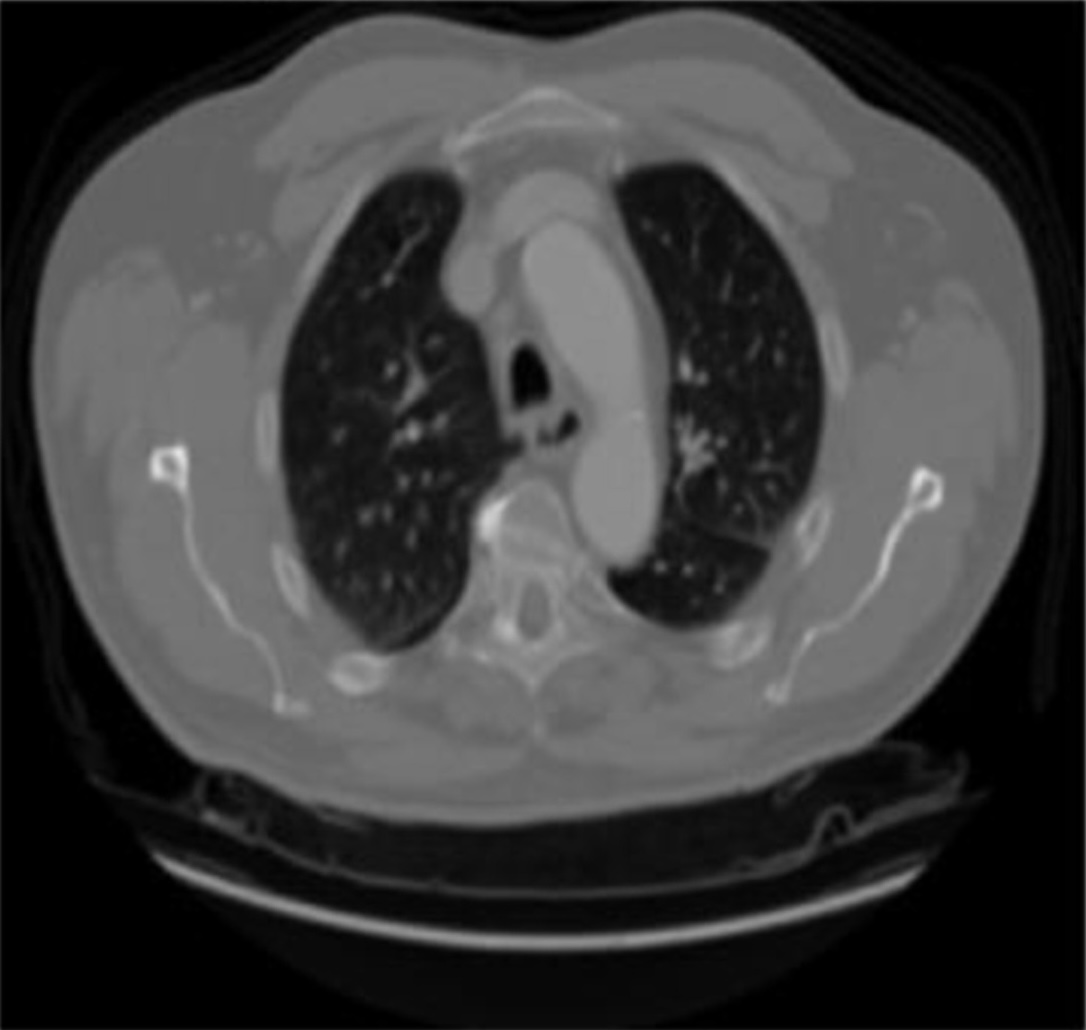
\includegraphics[width=0.5\textwidth]{../assets/01-overview/lc-scc-ct.jpg}

    \small\textit{CT scan of patient diagnosed with lung Squamous Cell Carcinoma. 
    \cite{SHATNAWI2025100188}}
\end{center}
\vspace{1em}

\begin{itemize}
    % Large Cell Carcinoma: aggressive, poorly differentiated
    \item \textbf{Large Cell Carcinoma}: A heterogeneous group of poorly differentiated tumors 
    lacking glandular or squamous characteristics. It is often aggressive and located in peripheral 
    lung tissue. The WHO/IASLC classification includes variants such as large cell neuroendocrine 
    carcinoma (LCNEC), basaloid carcinoma, and large cell carcinoma with rhabdoid phenotype. 
    \cite{nlm2025}
\end{itemize}

% CT scan image of large cell carcinoma
\vspace{1em}
\begin{center}
    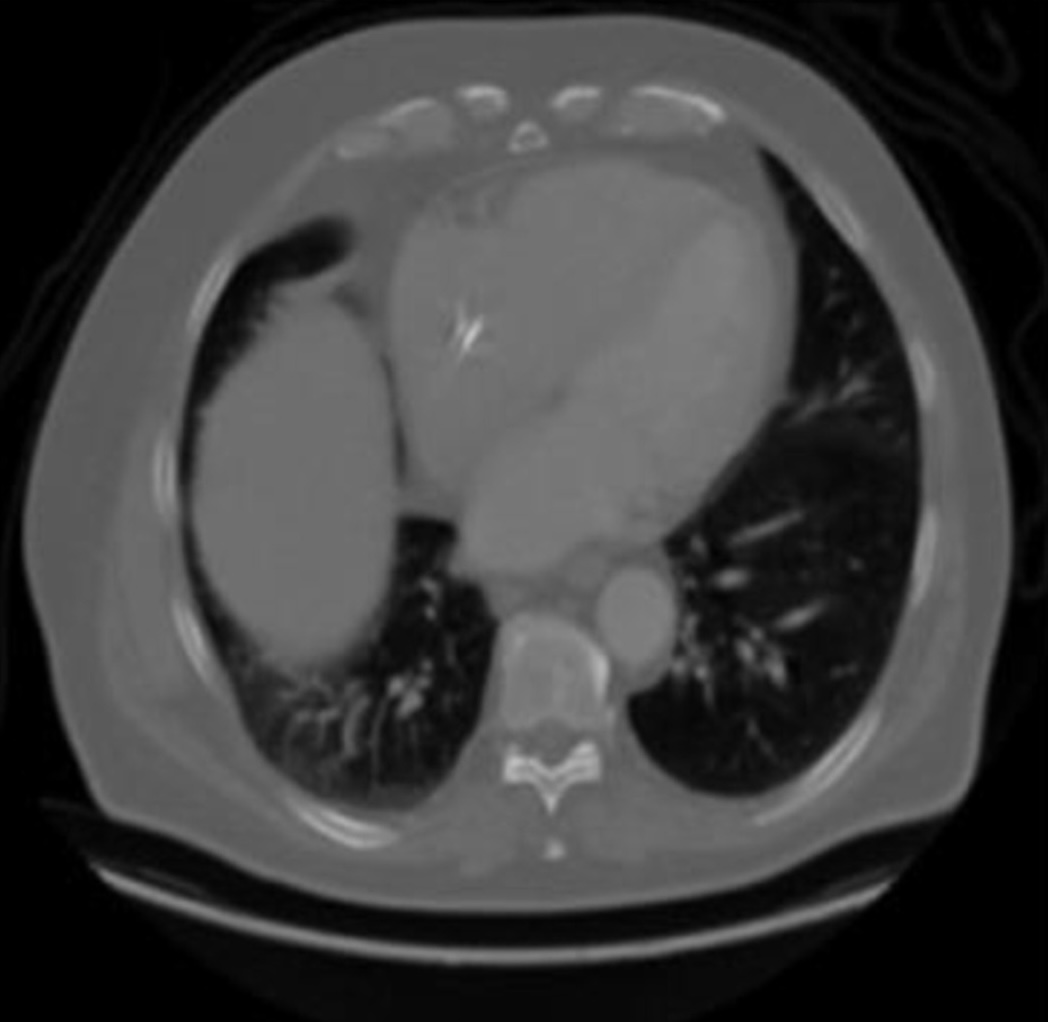
\includegraphics[width=0.5\textwidth]{../assets/01-overview/lc-lcc-ct.jpg}

    \small\textit{CT scan of patient diagnosed with lung Large Cell Carcinoma. 
    \cite{SHATNAWI2025100188}}
\end{center}
\vspace{1em}

\begin{itemize}
    % Other rare NSCLC subtypes
    \item \textbf{Others}: This category encompasses a diverse group of rare or poorly 
    differentiated NSCLC histologies.
    
    % Mixed subtype with both adenocarcinoma and squamous features
    \textit{Adenosquamous carcinoma} exhibits both glandular (adenocarcinoma) and squamous 
    components, and is typically more aggressive than either component alone.
    
    % Rare and aggressive tumors with sarcoma-like appearance
    \textit{Sarcomatoid carcinomas} are poorly differentiated tumors that show sarcoma-like features 
    and include pleomorphic carcinoma, spindle cell carcinoma, and giant cell carcinoma. These are 
    rare and generally associated with a poor prognosis.
    
    % Salivary gland-like tumors
    \textit{Salivary gland-type tumors}, such as mucoepidermoid carcinoma and adenoid cystic 
    carcinoma, are histologically similar to tumors of the salivary glands and are extremely rare in 
    the lungs.
    
    % Neuroendocrine origin, usually low-grade
    \textit{Carcinoid tumors} are neuroendocrine in origin and tend to be less aggressive, although 
    atypical variants can exhibit more malignant behavior.
    
    % Unclassified tumors due to lack of clear histological identity
    Finally, some tumors remain \textit{unclassified} due to ambiguous histological features or 
    inadequate sampling, and are grouped as NSCLC not otherwise specified (NOS). \cite{travis2015}
\end{itemize}

% NSCLC subtype distribution chart
\vspace{1em}
\begin{center}
    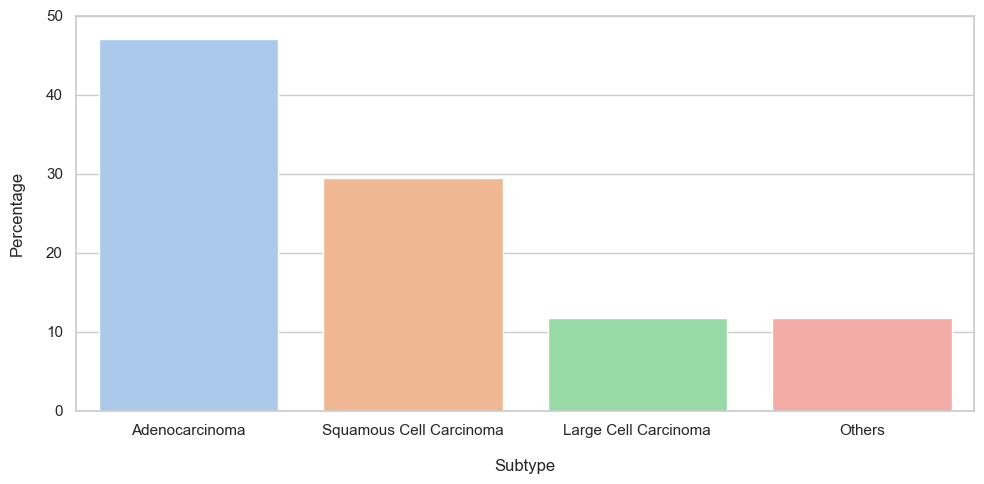
\includegraphics[width=1.00\textwidth]{../assets/01-overview/nsclc-dist.png}

    \small\textit{Distribution of NSCLC histological subtypes. Data source: \cite{nlm2025}}.
\end{center}
\vspace{1em}

% Description of Small Cell Lung Cancer (SCLC)
\textbf{SCLC}, in contrast, tends to grow rapidly and spread early to distant body sites. It is 
strongly associated with cigarette smoking and is often diagnosed at an advanced stage.

% --------------------------------------------------------------------------------------------------
% Subsection: Epidemiology and Global Burden
% --------------------------------------------------------------------------------------------------
\subsection{Epidemiology and Global Burden}
% Global impact and mortality rate
Lung cancer remains one of the leading causes of cancer-related deaths worldwide. According to the 
World Health Organization (WHO), lung cancer causes approximately 1.8 million deaths annually, 
making it the most lethal form of cancer. \cite{who2024}

\begin{itemize}
    % Incidence varies by region and development level
    \item \textbf{Incidence}: Varies globally, significantly depending by region, often reflecting 
    differences in tobacco use, environmental exposure, and socioeconomic status. High-income 
    countries generally show declining trends in incidence due to successful tobacco control 
    efforts, while many low and middle-income countries are seeing rising rates due to increased 
    smoking prevalence and industrial pollution.
\end{itemize}

% Global incidence map
\vspace{1em}
\begin{center}
    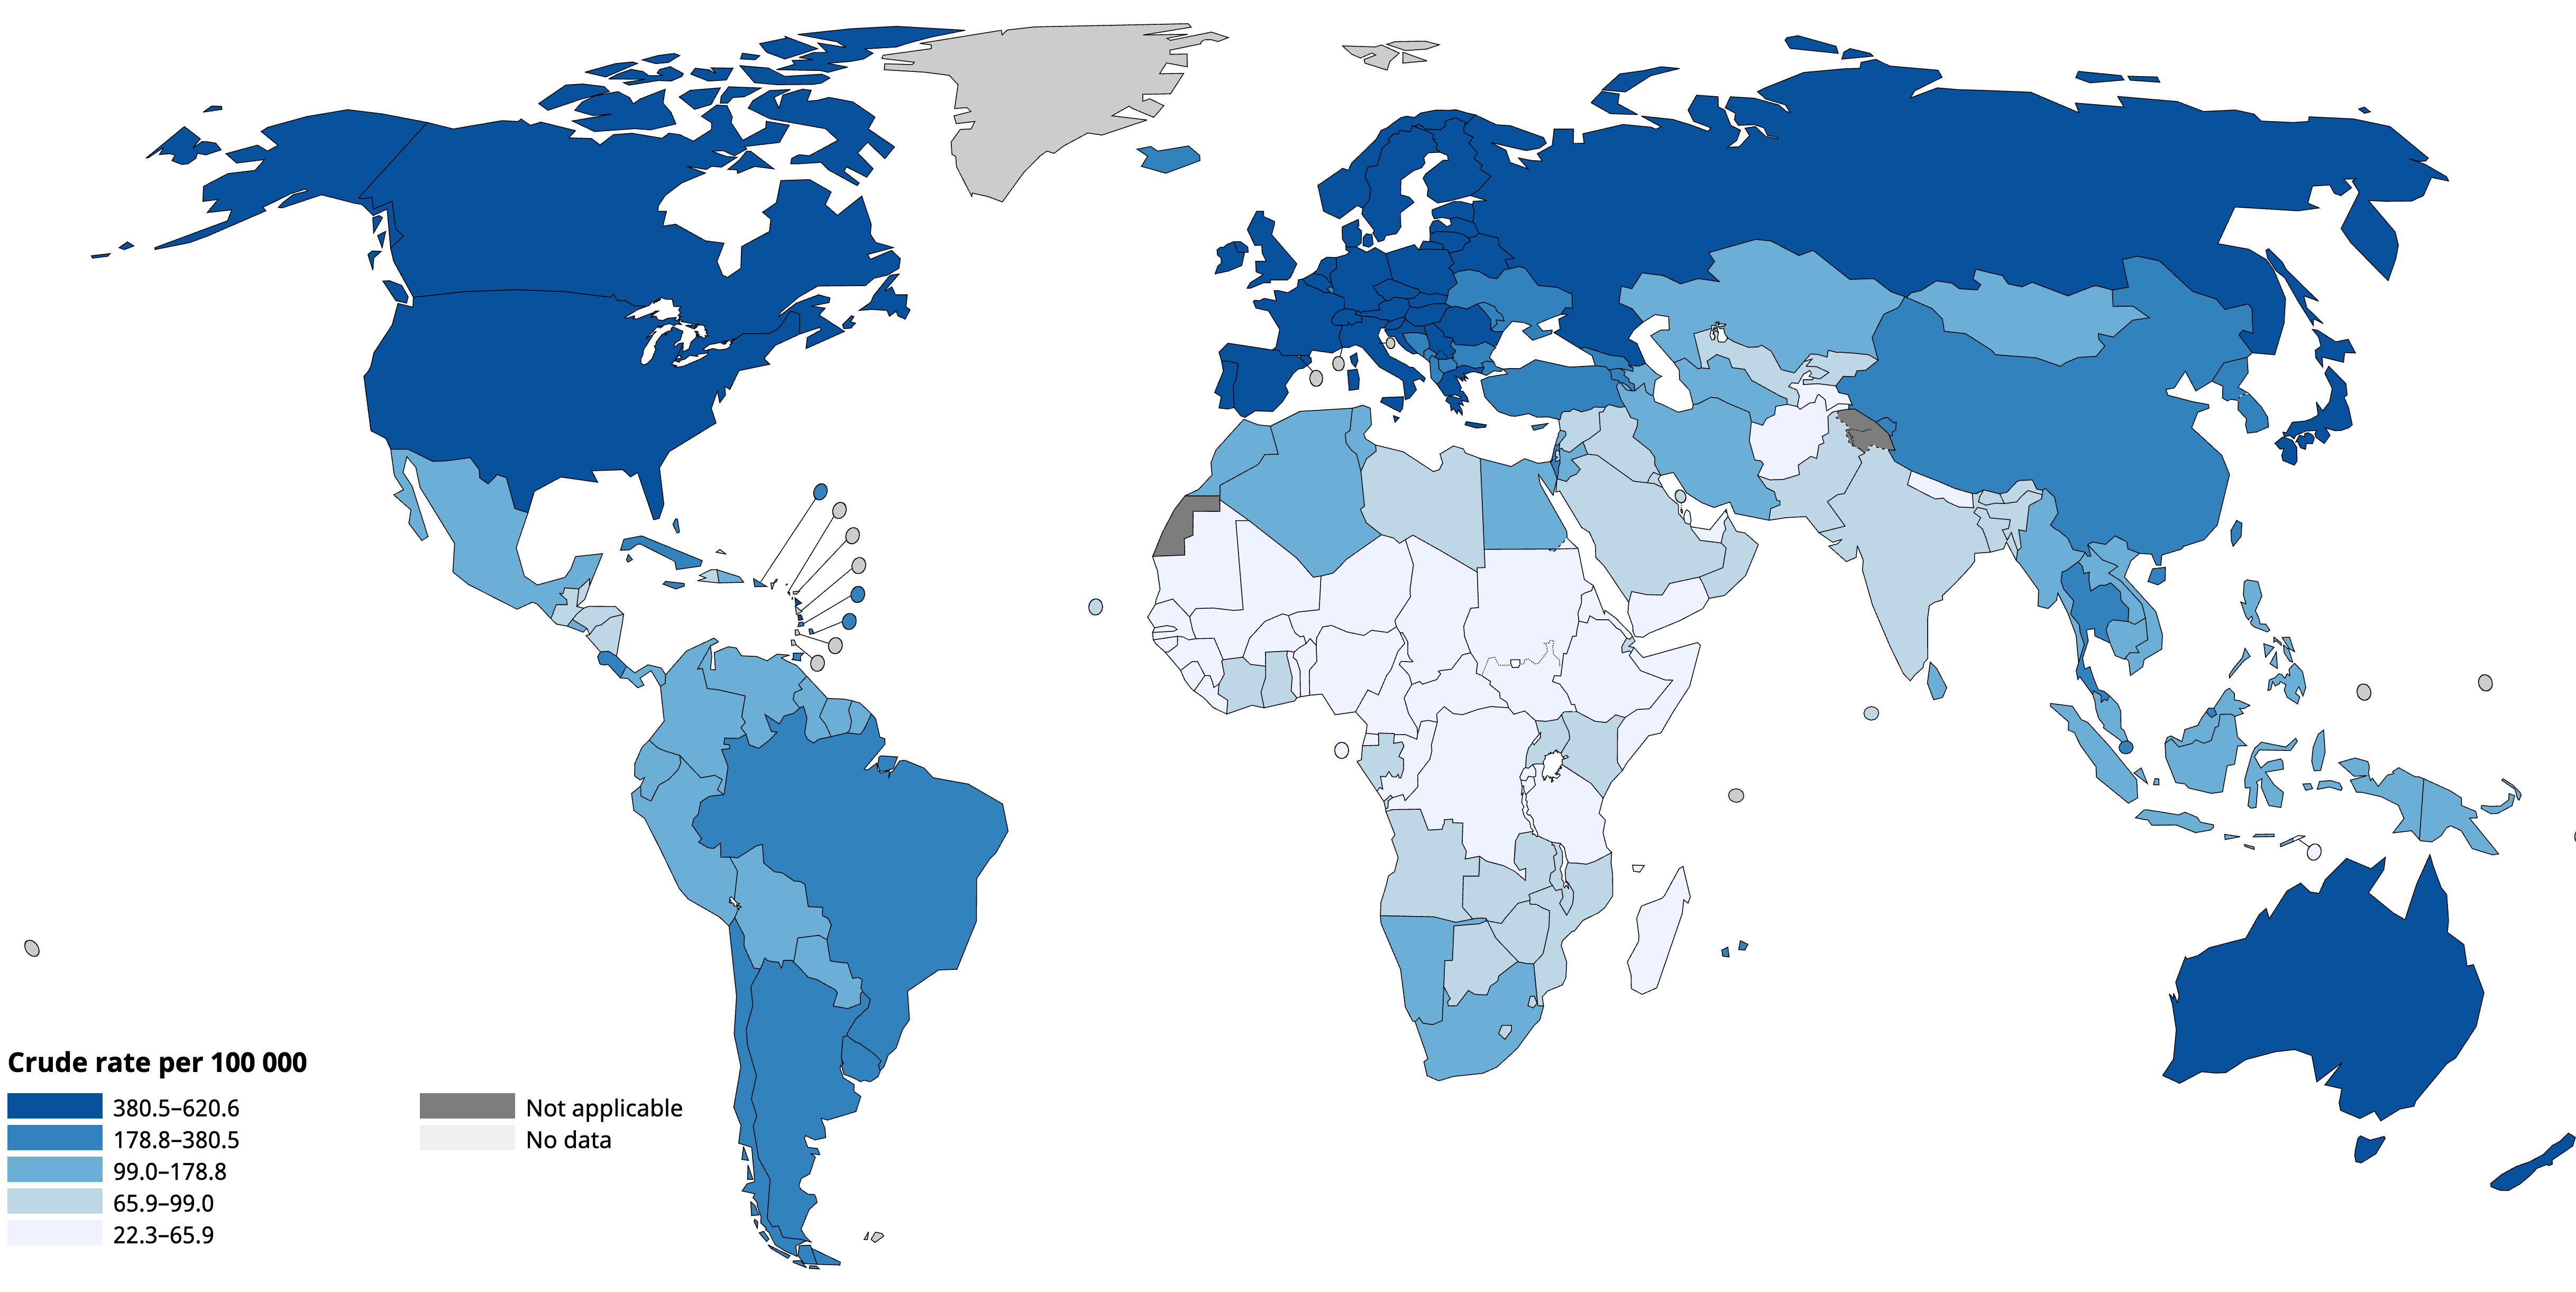
\includegraphics[width=1.00\textwidth]{../assets/01-overview/lc-crude-rate.png}

    \small\textit{Lung cancer estimated incidence crude rate (per 100.000 people). \cite{who2024}}
\end{center}
\vspace{1em}

\begin{itemize}
    % Gender-based differences in lung cancer rates
    \item \textbf{Gender Distribution}: Historically more prevalent in men, but the gap is narrowing 
    due to increased smoking rates among women over time. Biological differences, including hormonal 
    and genetic factors, may also contribute to distinct patterns of disease development and 
    progression between sexes.
\end{itemize}

% Death rate comparison by gender
\vspace{1em}
\begin{center}
    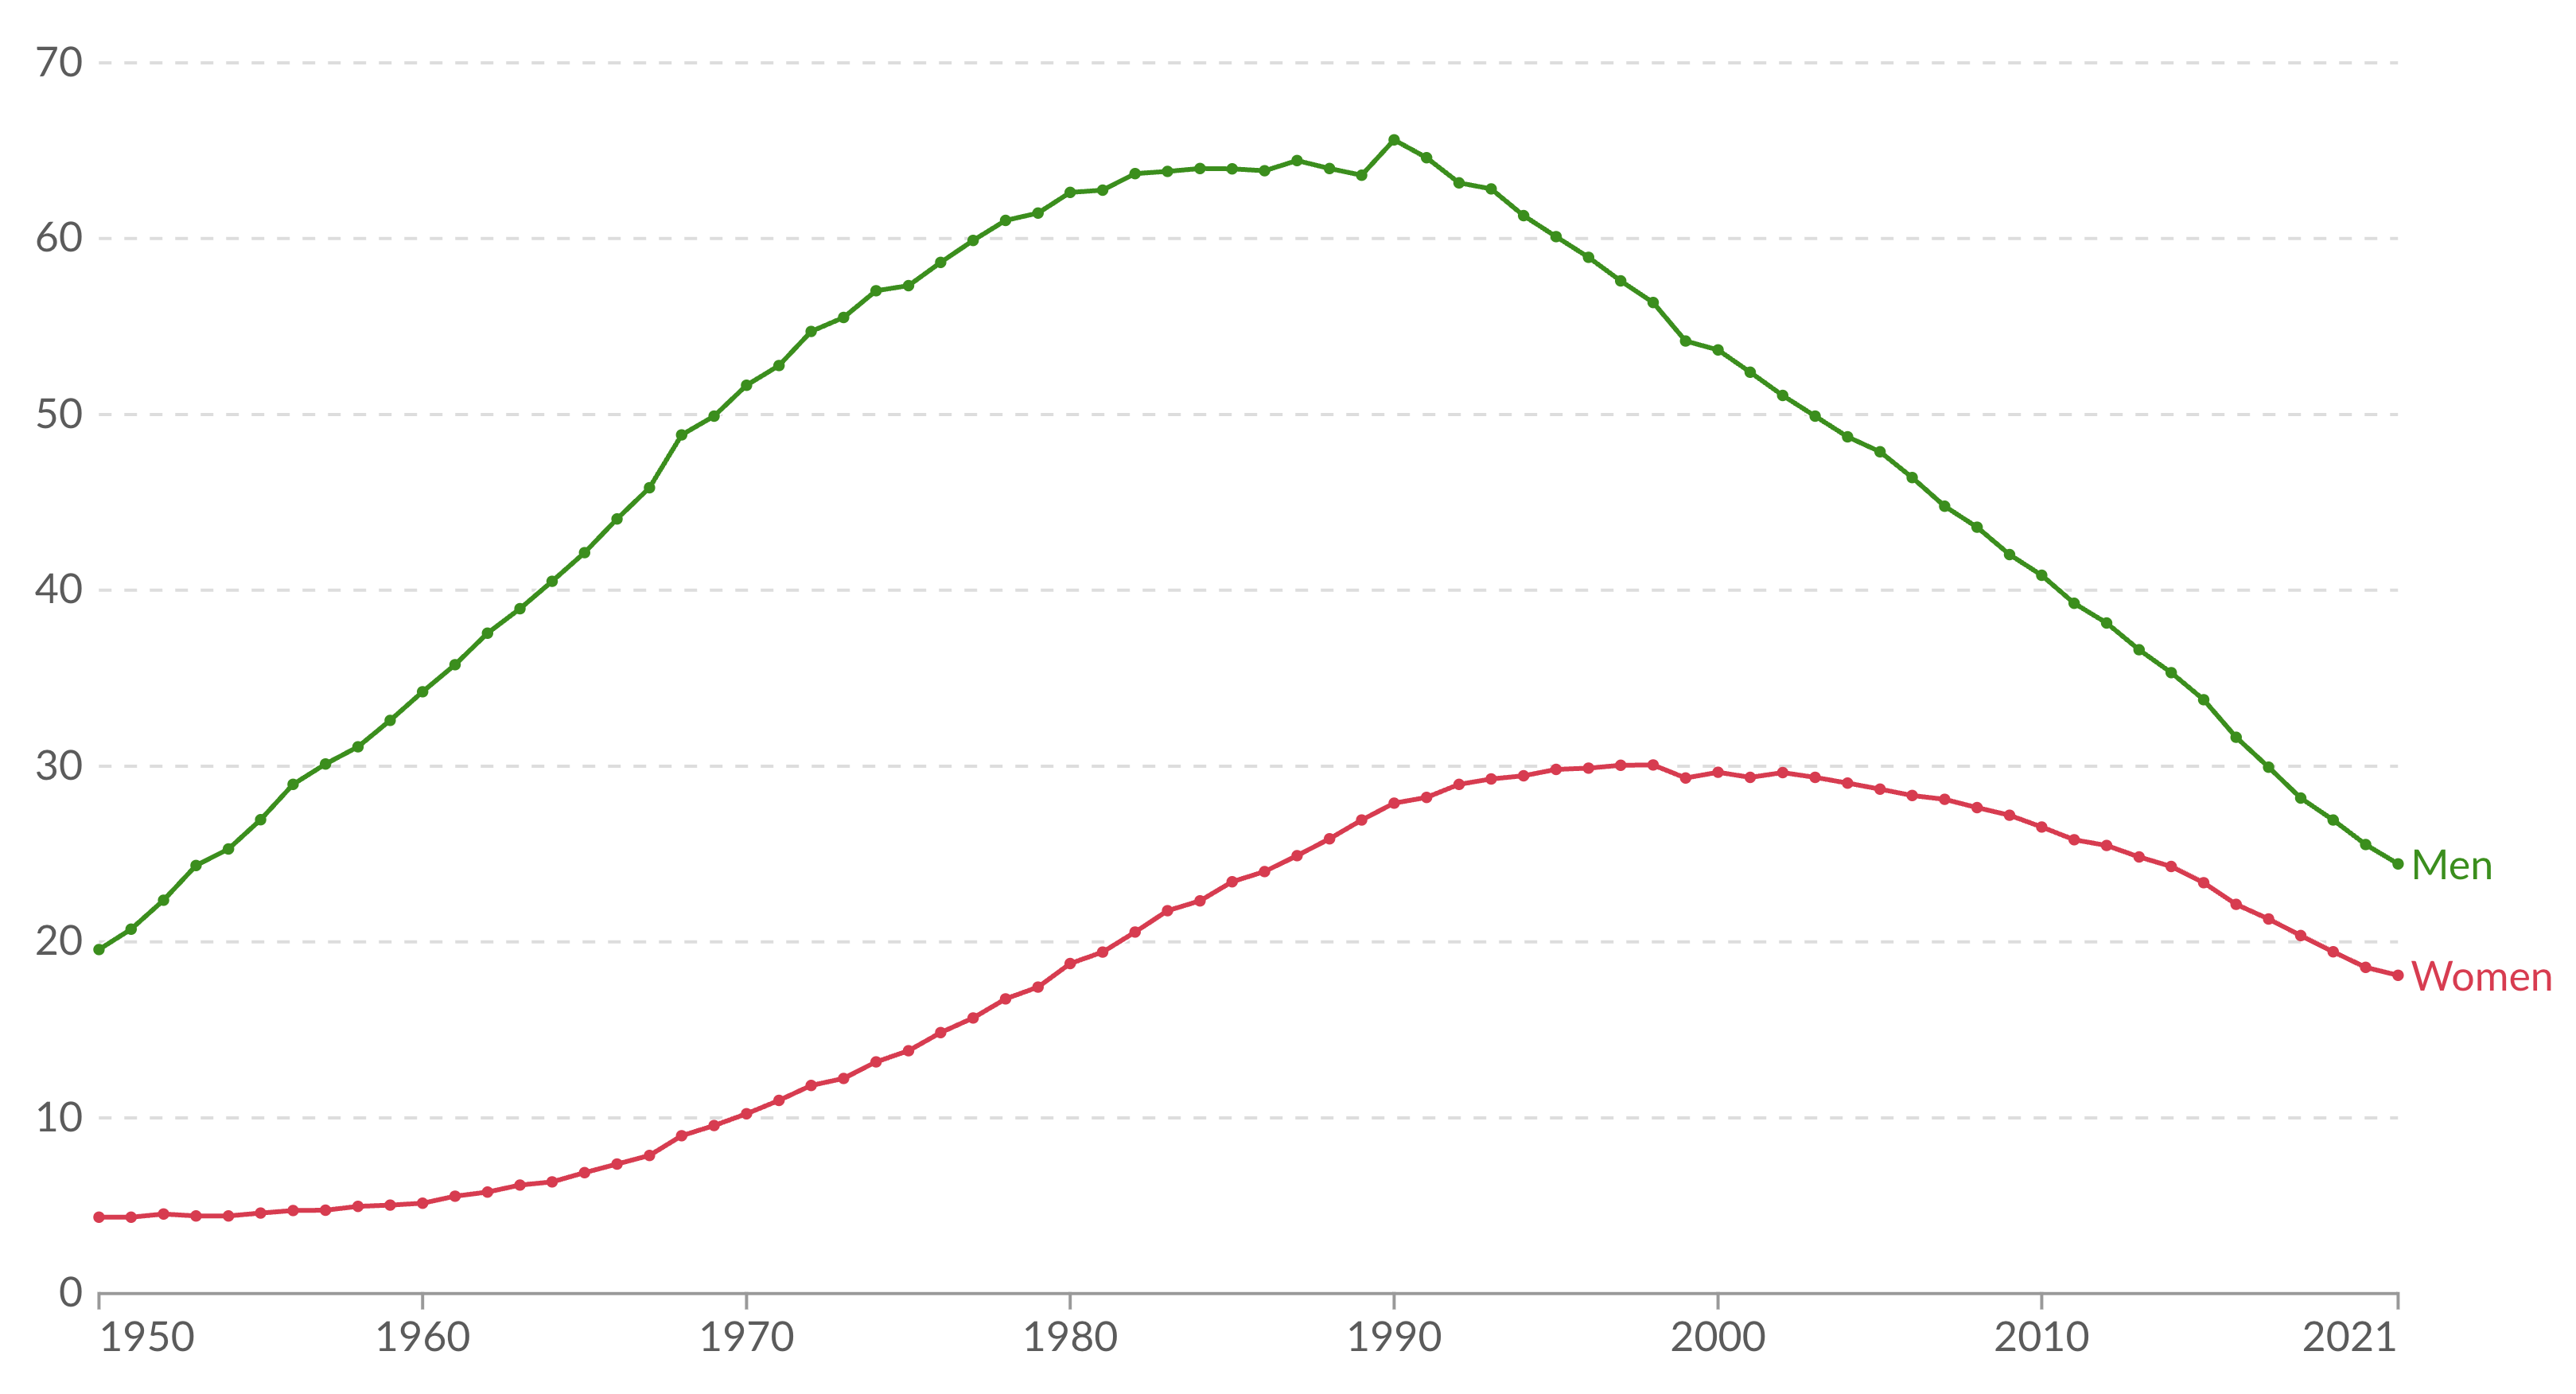
\includegraphics[width=1.00\textwidth]{../assets/01-overview/lc-death-men-vs-women.png}
    \small\textit{Lung cancer death rates (per 100.000 people). \cite{ourworldindata, who2024}}
\end{center}
\vspace{1em}

\begin{itemize}
    % Survival rates and prognosis differences
    \item \textbf{Survival Rates}: The 5-year survival rate remains low (around 20\%) 
    \cite{nlm2025}, especially for cases diagnosed at a late stage. Mortality closely mirrors 
    incidence rates, with lung cancer accounting for nearly one in five cancer deaths. Non-small 
    cell lung cancer (NSCLC), the most common type, generally has better outcomes than small cell 
    lung cancer (SCLC), especially when diagnosed early.
\end{itemize}

% Mortality risk chart
\vspace{1em}
\begin{center}
    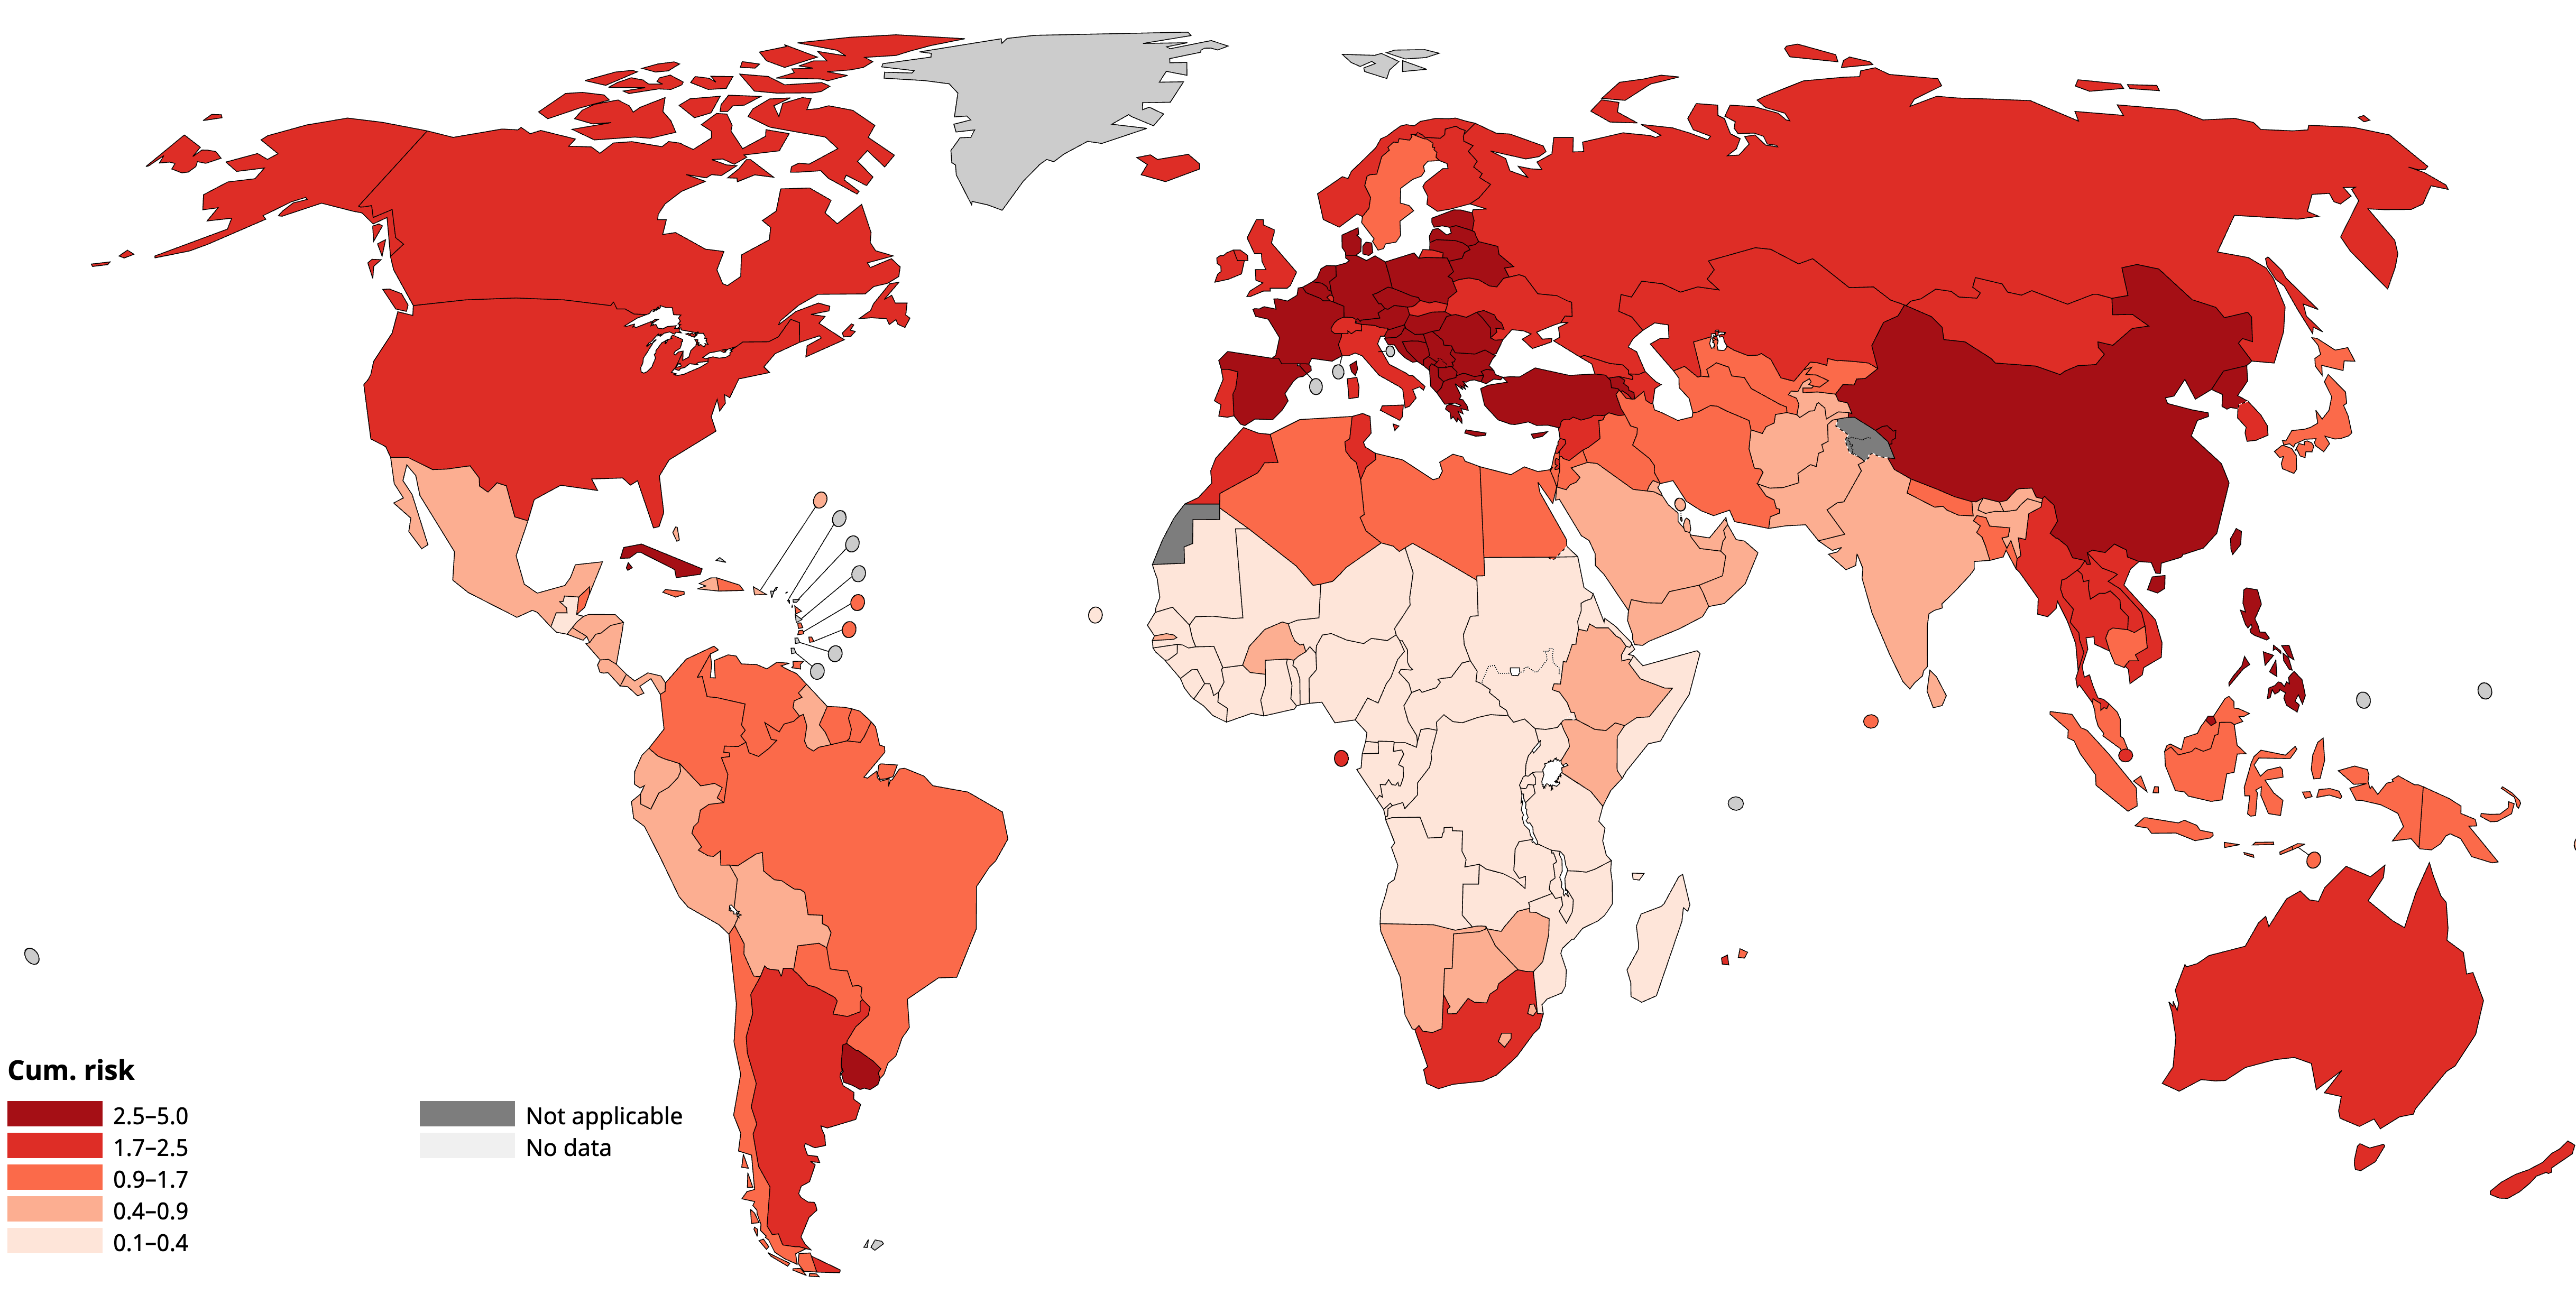
\includegraphics[width=1.00\textwidth]{../assets/01-overview/lc-cumulative-risk.png}

    \small\textit{Lung cancer estimated mortality cumulative risk (per 100.000 people). 
    \cite{who2024}}
\end{center}
\vspace{1em}

% Final statement about the global impact
The global burden of lung cancer is not only reflected in mortality rates but also in the economic 
and social costs of treatment and loss of productivity. Prevention and early detection remain 
critical in reducing this burden.
